%\documentclass[]{beamer}
\documentclass[aspectratio=169,tikz]{beamer}
%\pdfpkresolution=3600
\usepackage[utf8]{inputenc} % use UTF-8
\usepackage[T2A,OT1]{fontenc} % rus fonts
\usepackage[russian]{babel}

\usepackage{xspace}
\usepackage{lipsum}
\usepackage{standalone}
\usepackage{setspace}
\usepackage{tkz-euclide}
\usepackage{subfigure}
\usepackage{listings} % for code listings

\usetikzlibrary{shapes,backgrounds}
\usepackage{pgf-umlcd}

\tikzstyle{startstop} = [rectangle, rounded corners, minimum width=3cm, minimum height=1cm,text centered, draw=black, fill=red!30]

\tikzstyle{io} = [trapezium, trapezium left angle=70, trapezium right angle=110, minimum width=3cm, minimum height=1cm, text centered, draw=black, fill=blue!30]

\tikzstyle{process} = [rectangle, minimum width=3cm, minimum height=1cm, text centered, draw=black, fill=orange!30]

\tikzstyle{decision} = [diamond, minimum width=3cm, minimum height=1cm, text centered, draw=black, fill=green!30]

\tikzstyle{arrow} = [thick,->,>=stealth]


\usepackage{tkz-euclide}
\usetikzlibrary{shapes,backgrounds}


\tikzset{weird fill/.style={append after command={
			\pgfextra
			\draw[sharp corners, fill=#1,fill opacity=0.3, draw=none]% 
			(\tikzlastnode)% 
			[rounded corners=8pt] -| (\tikzlastnode.west)
			[rounded corners=8pt] |- (\tikzlastnode.north)% 
			[rounded corners=8pt] -| (\tikzlastnode.east)% 
			[rounded corners=8pt] |- (\tikzlastnode.south);
			\endpgfextra}}}

\newcommand\pack[6][]{%
	\path[#1] (#4,#5) -- (#4-#2 , #5)
	-- (#4-#2 ,#5+#3) -- (#4-#2 ,#5+#3 + 0.7)
	-- (#4-#2 + #6 * #2 ,#5+#3 + 0.7) -- (#4-#2 + #6 * #2+0.0 ,#5+ #3)
	-- (#4, #5+#3)
	--cycle;
	\path[#1] (#4-#2 , #5+ #3) -- (#4-#2 + 0.8* #2+0.5 ,#5+ #3);
}

\def\package[#1](#2:#3:#4:#5:#6){%
	% Synopsis                 2  3 4 5 6
	% \package[draw options](text:w:h:x:y)
	%	\pack[draw=black, rounded corners=8pt, thick, fill=white]{#3}{#4}{#5}{#6};
	%	\pack[draw=black, rounded corners=8pt, thick, fill opacity=0.2, #1]{#3}{#4}{#5}{#6};
	%	\node [anchor=west, draw=black, thick] at (#5-#3,  #6+#4+0.35) {\texttt{#2}};	
	
	%	\node [anchor=west] at (#5-#3,  #6+#4+0.35) {\texttt{#2}};
	\draw node[minimum height=5mm,anchor=south west,minimum width=15mm,
	append after command={[rounded corners=8pt](b.west)|-(b.north)},
	append after command={[rounded corners=8pt](b.north)-|(b.east)},
	append after command={[rounded corners=0pt](b.east)|-(b.south)},
	append after command={[rounded corners=0pt](b.south)-|(b.west)}, weird fill=#1]
	(b) at (#5,  #6+#4) {\texttt{#2}};
	
	\draw node[minimum height=5mm,anchor=south west,minimum width=15mm,
	append after command={[rounded corners=8pt](b.west)|-(b.north)},
	append after command={[rounded corners=8pt](b.north)-|(b.east)},
	append after command={[rounded corners=0pt](b.east)|-(b.south)},
	append after command={[rounded corners=0pt](b.south)-|(b.west)}]
	(c) at (#5,  #6+#4) {\texttt{#2}};
	
	
	\path[draw,black,fill=#1,fill opacity=0.3,rounded corners=8pt] (#5, #6 + #4) -- (#5,#6) -- (#5+#3, #6) -- (#5+#3, #6 + #4) -- (#5, #6 + #4);
}



\newcolumntype{Z}{>{\centering\let\newline\\\arraybackslash\hspace{0pt}}X} 
\newcolumntype{M}{>{\raggedright\let\newline\\\arraybackslash\hspace{0pt}}X}
\newcolumntype{L}[1]{>{\raggedright\let\newline\\\arraybackslash\hspace{0pt}}m{#1}}
\newcolumntype{C}[1]{>{\centering\let\newline\\\arraybackslash\hspace{0pt}}m{#1}}

\newcommand{\kmeans}{\mbox{$ k $-means}\xspace}
\newcommand{\Ward}{Ward\xspace}
\newcommand{\AWard}{\mbox{A-Ward}\xspace}
\newcommand{\Wardp}{\mbox{Ward$ _p $}\xspace}
\newcommand{\AWardpb}{\mbox{A-Ward$ _{p\beta} $}\xspace}
\newcommand{\BisectingKmeans}{Bisecting \mbox{k-means}\xspace}
\newcommand{\BiKMR}{\mbox{BiKM-R}\xspace}
\newcommand{\dePDDP}{dePDDP\xspace}
\newcommand{\ikmeans}{\mbox{$ ik $-means}\xspace}
\newcommand{\imwkmeanspb}{\mbox{$ imwk $-means$ _{p\beta} $}\xspace}
\newcommand{\PDDP}{PDDP\xspace}


%\renewcommand{\raggedright}{\leftskip=0pt \rightskip=0pt plus 0cm}
\hyphenpenalty=100000 %%% to turn the hyphenation off

\usetheme[progressbar=frametitle]{metropolis}

\newcommand{\myitem}{\item[\color{blue}$ \rhd $]}
\newcommand{\sitem}{\item[$ \ast $]}
%%%%%%%%%%%%%%%%%%%%%%%%%%%%%%%%%%%%%%%%%%%%%%%%%%%%%%%%%%%%%%%%%%%%%%%%%%%
 
 \usepackage{tkz-euclide}
 \usetikzlibrary{shapes,backgrounds}
 
 \newcommand\Star[3][]{%
 	\path[#1] (0  :#3) -- ( 36:#2) 
 	-- (72 :#3) -- (108:#2)
 	-- (144:#3) -- (180:#2)
 	-- (216:#3) -- (252:#2)
 	-- (288:#3) -- (324:#2)--cycle;
 }
 \newcommand\Center[3][]{
 	\begin{scope}[shift = {(#2,#3)}, scale=0.08]
 		\Star[#1]{2}{4}
 	\end{scope}
 }
 
 \newcommand\point[3][]{
 	\begin{scope}[shift = {(#2,#3)}, scale=0.08]
 		\draw[#1] (0,0) circle (1.5);
 	\end{scope}
 }

\newcommand\pointt[3][]{
	\begin{scope}[shift = {(#2,#3)}, scale=0.08/0.6]
		\draw[#1] (0,0) circle (1.5);
	\end{scope}
} 

\newcommand\pointtt[3][]{
	\begin{scope}[shift = {(#2,#3)}, scale=0.08/0.5]
		\draw[#1] (0,0) circle (1.5);
	\end{scope}
}
%%%%%%%%%%%%%%%%%%%%%%%%%%%%%%%%%%%%%%%%%%%%%%%%%%%%%%%%%%%%%%%%%%%%%%%%%%%

\title{Разработка программного обеспечения, ориентированного на пользователя, для проведения кластер-анализа по критерию наименьших квадратов}

\author[Еремейкин П.А. \& Миркин Б.Г.]{
	\texorpdfstring{
	\begin{columns}
		\column{.45\linewidth}
		\raggedleft
		\begin{flushleft}
			Выполнил:\\
			Еремейкин Пётр Александрович\\
			студент группы мНоД16-ТМСС\\
			\href{mailto:eremeykin@gmail.com}{\texttt{eremeykin@gmail.com}}
		\end{flushleft}
		\column{.45\linewidth}
		\begin{flushright}
			Руководитель:\\
			Миркин Борис Григорьевич\\
			д.т.н. профессор\\
			\vspace*{1\baselineskip} 
		\end{flushright}
	\end{columns}
	}
	{Еремейкин \& Миркин}
}
\institute{\vspace{1cm} НИУ ВШЭ\\Июнь 2018}
\date{}



\begin{document}
	\usetikzlibrary{shapes,backgrounds}
	\usetikzlibrary{arrows.meta}
	\usetikzlibrary{snakes}
	
	\begin{frame}
		\titlepage
	\end{frame}
	
	\begin{frame}{Постановка задачи кластеризации}		
		\parbox{\linewidth}{
			\textbf{Дано: }  $ Y $ --- множество из $ N $ объектов, характеризующихся $ V $ признаками
			}
		\begin{equation*}
			Y= \begin{pmatrix} 
			y_{1} \\
			\cdots \\ 
			y_{N} 
			\end{pmatrix}
			= \begin{pmatrix} 
			y_{11} & \cdots  & y_{1V} \\ 
			\cdots & \cdots  & \cdots \\ 
			y_{N1} & \cdots  & y_{NV} 
			\end{pmatrix}
		\end{equation*}
		\parbox{\linewidth}{
			\textbf{Найти: }  разбиение $ S = \{C_1,\ldots,C_K\} $, из $ K $ кластеров,\\
			\begin{columns}
			\column{0.65\linewidth}
			\begin{equation*}
				\bigcup_{k=1}^{K}C_k=Y
			\end{equation*}
			
			\begin{equation*}
				 C_{k1} \cap C_{k2}=\varnothing ,\:k1 \neq k2
			\end{equation*}
			\column{0.35\linewidth}
			\begin{figure} % \ContinuedFloat
				\centering
				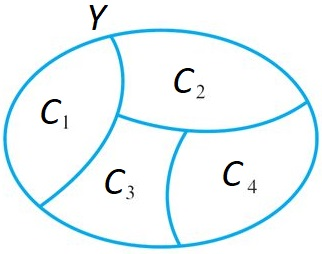
\includegraphics[width=0.70\linewidth]{img/partition}
			\end{figure}
			\end{columns}
		}
	\end{frame}

	\begin{frame}[t]{Программная система INDACT}
	\vspace{-0.1cm}
	\begin{center}
		\LARGE  \textbf{INDACT:}
		{ \textbf{IN}telligent \textbf{DA}ta \textbf{C}lustering \textbf{T}oolkit\\}
	\end{center}
	\vspace{0.1cm}
	\normalsize
	Система для кластерного анализа данных\\
	($ \sim 5000 $ объектов, $ \sim 30 $ признаков)
	\begin{itemize}
		\item \textbf{Язык:} Python 3
		\item \textbf{Пользовательский интрефейс:} оконный графический (PyQt, Matplotlib)
		\item \textbf{Состав:} 5 новейших алгоритмов кластеризации
		\item \textbf{Библиотеки:} Pandas, NumPy, SciPy, scikit-learn 
		\item \textbf{Тестирование:} pytest
		\item \textbf{Дистрибуция:} pyinstaller
	\end{itemize}
	\end{frame}
	
	\begin{frame}{Состав системы INDACT}
	\begin{itemize}
		\item Графический интерфейс
		\item Библиотека алгоритмов:
		\begin{itemize}
			\sitem нормализация
			\sitem кластер-анализ
			\sitem подготовка отчётов
			\sitem проведение вычислительных экспериментов
		\end{itemize}
		
	\end{itemize}
	\end{frame}
	
	\begin{frame}{Пользовательский графический интерфейс}
	\begin{columns}
	\column{0.2\linewidth}
	\begin{figure}[T] % \ContinuedFloat
		\centering
		\includestandalone[width=0.9\linewidth]{img/tikz/stages-vertical-norm}
	\end{figure}
	\column{0.8\linewidth}
	\begin{figure}[T] % \ContinuedFloat
		\begin{tikzpicture}
		\node[anchor=south west,inner sep=0] (image) at (0,0) {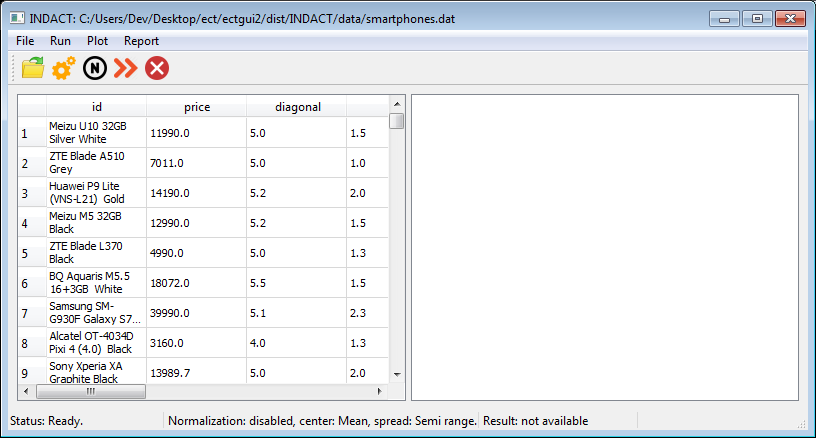
\includegraphics[width=0.95\linewidth]{img/diploma/instruction/load-result-2}};
		\node[anchor=south west,inner sep=0] (image) at (3,2) {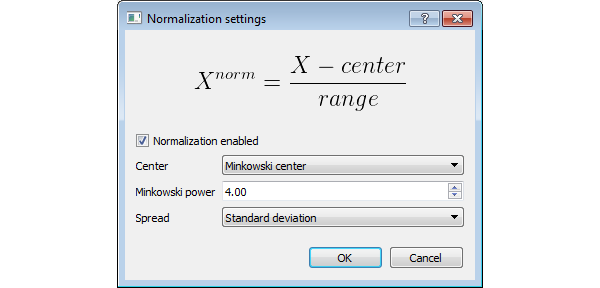
\includegraphics[width=0.60\linewidth]{img/diploma/instruction/mink-norm-params}};
		\end{tikzpicture}
	\end{figure}
	\end{columns}
	\end{frame}


	\begin{frame}{Недостатки алгоритмов кластеризации}
	
	\begin{columns}
		
		\column{0.58\linewidth}
		
		\begin{center}
			{\Huge \kmeans}
		\end{center}
		
		\parbox{\linewidth}{
			Поочерёдная минимизация квадратичного критерия по двум группам переменных: центрам кластеров и принадлежности объектов кластерам.
		}
		
		\vspace*{1\baselineskip} 
		\textbf{Недостатки:}
		\begin{itemize}
			\item число кластеров
			\item инициализация
			\item неточности в данных\\ (лишние признаки, объекты и пр.)
		\end{itemize}
		
		\column{0.38\linewidth}
		\centering
		\vspace{-.4cm}
		\begin{figure} % \ContinuedFloat
			\centering
			\includestandalone[width=\linewidth]{img/tikz/k-means-demo}
		\end{figure}
	\end{columns} 
	
	\end{frame}

	\begin{frame}{Алгоритмы}
	
	\begin{columns}
		\column{0.2\linewidth}
		\begin{minipage}[c][8cm][c]{\linewidth}
			\begin{itemize}
				\item \ikmeans \tikz[remember picture] \node[coordinate, xshift=0.1cm,yshift=0.5em] (n1) {};
				\item \dePDDP
				\item \BiKMR \tikz[remember picture] \node[coordinate, xshift=0.1cm,] (n2) {};
				\hspace{2cm}
				\item \AWard \tikz[remember picture] \node[coordinate, xshift=0.3cm,yshift=0.5em] (t1) {};
				\item \AWardpb   \tikz[remember picture] \node[coordinate, xshift=0.3cm,] (t2) {};
			\end{itemize}
			\hrule
			{\tiny Алгоритмы разработаны Миркиным et al. \par}
			\begin{tikzpicture}[overlay,remember picture]
			\path (n2) -| node[coordinate] (p3) {} (n1);
			\draw[thick,decorate,decoration={brace,amplitude=3pt}]
			(n1) -- (p3) node[midway, right=4pt] {Дивизивные};
			
			\path (t2) -| node[coordinate] (p3) {} (t1);
			\draw[thick,decorate,decoration={brace,amplitude=3pt}]
			(t1) -- (p3) node[midway, right=4pt] {Агломеративные};
			\end{tikzpicture}
		\end{minipage}
		
		\column{0.8\linewidth}
		%		\begin{figure} % \ContinuedFloat
		%			\centering
		%			\includestandalone[height=0.9\textheight]{img/tikz/alg-types2}
		%		\end{figure}
	\end{columns}			
	\end{frame}
	
	\begin{frame}{Алгоритмы}
	
	\begin{columns}
	\column{0.2\linewidth}
	\begin{minipage}[c][8cm][c]{\linewidth}
		\begin{itemize}
			\item \ikmeans \tikz[remember picture] \node[coordinate, xshift=0.1cm,yshift=0.5em] (n1) {};
			\item \dePDDP
			\item \BiKMR \tikz[remember picture] \node[coordinate, xshift=0.1cm,] (n2) {};
			\item \AWard \tikz[remember picture] \node[coordinate, xshift=0.3cm,yshift=0.5em] (t1) {};
			\item \AWardpb   \tikz[remember picture] \node[coordinate, xshift=0.3cm,] (t2) {};
		\end{itemize}			
		\hrule
		{\tiny Алгоритмы разработаны Миркиным et al. \par}
		\begin{tikzpicture}[overlay,remember picture]
		\path (n2) -| node[coordinate] (p3) {} (n1);
		\draw[thick,decorate,decoration={brace,amplitude=3pt}]
		(n1) -- (p3) node[midway, right=4pt] {\color{blue}\textbf{Дивизивные}};
		
		\path (t2) -| node[coordinate] (p3) {} (t1);
		\draw[thick,decorate,decoration={brace,amplitude=3pt}]
		(t1) -- (p3) node[midway, right=4pt] {Агломеративные};
		\end{tikzpicture}
	\end{minipage}
	
	\column{0.8\linewidth}
	\begin{figure} % \ContinuedFloat
		\centering
		\includestandalone[height=0.9\textheight]{img/tikz/alg-types1}
	\end{figure}
	\end{columns}			
	\end{frame}
	
	\begin{frame}{Алгоритмы}
	
	\begin{columns}
	\column{0.2\linewidth}
	\begin{minipage}[c][8cm][c]{\linewidth}
	\begin{itemize}
		\item \ikmeans \tikz[remember picture] \node[coordinate, xshift=0.1cm,yshift=0.5em] (n1) {};
		\item \dePDDP
		\item \BiKMR \tikz[remember picture] \node[coordinate, xshift=0.1cm,] (n2) {};
		\item \AWard \tikz[remember picture] \node[coordinate, xshift=0.3cm,yshift=0.5em] (t1) {};
		\item \AWardpb   \tikz[remember picture] \node[coordinate, xshift=0.3cm,] (t2) {};
	\end{itemize}
	\hrule
	{\tiny Алгоритмы разработаны Миркиным et al. \par}
	\begin{tikzpicture}[overlay,remember picture]
	\path (n2) -| node[coordinate] (p3) {} (n1);
	\draw[thick,decorate,decoration={brace,amplitude=3pt}]
	(n1) -- (p3) node[midway, right=4pt] {Дивизивные};
	
	\path (t2) -| node[coordinate] (p3) {} (t1);
	\draw[thick,decorate,decoration={brace,amplitude=3pt}]
	(t1) -- (p3) node[midway, right=4pt] {\color{blue}\textbf{Агломеративные}};
	\end{tikzpicture}
	\end{minipage}
	
	\column{0.8\linewidth}
	\begin{figure} % \ContinuedFloat
	\centering
	\includestandalone[height=0.9\textheight]{img/tikz/alg-types2}
	\end{figure}
	\end{columns}			
	\end{frame}
	
	\begin{frame}{Алгоритмы}
	
	\begin{columns}
	
	\column{0.20\linewidth}
	\begin{minipage}[c][8cm][c]{\linewidth}
	\begin{itemize}
	\myitem {\color{blue}\textbf{\ikmeans}} \tikz[remember picture] \node[coordinate, xshift=-0.03cm,yshift=0.5em] (n1) {};
	\item \dePDDP
	\item \BiKMR \tikz[remember picture] \node[coordinate, xshift=0.1cm,] (n2) {};
	\item \AWard \tikz[remember picture] \node[coordinate, xshift=0.3cm,yshift=0.5em] (t1) {};
	\item \AWardpb   \tikz[remember picture] \node[coordinate, xshift=0.3cm,] (t2) {};
	\end{itemize}
	\hrule
	{\tiny Алгоритмы разработаны Миркиным et al. \par}
	\begin{tikzpicture}[overlay,remember picture]
	\path (n2) -| node[coordinate] (p3) {} (n1);
	\draw[thick,decorate,decoration={brace,amplitude=3pt}]
	(n1) -- (p3) node[midway, right=4pt] {Д};
	
	\path (t2) -| node[coordinate] (p3) {} (t1);
	\draw[thick,decorate,decoration={brace,amplitude=3pt}]
	(t1) -- (p3) node[midway, right=4pt] {А};
	\end{tikzpicture}
	\end{minipage}
	
	\column{0.8\linewidth}
	\begin{figure} % \ContinuedFloat
	\centering
	\includestandalone[width=0.9\linewidth]{img/tikz/ik-means/ik-means-2}
	\end{figure}
	\end{columns}		
	\end{frame}
	
	\begin{frame}{Алгоритмы}
	
	\begin{columns}
	
	\column{0.20\linewidth}
	\begin{minipage}[c][8cm][c]{\linewidth}
	\begin{itemize}
	\myitem {\color{blue}\textbf{\ikmeans}} \tikz[remember picture] \node[coordinate, xshift=-0.03cm,yshift=0.5em] (n1) {};
	\item \dePDDP
	\item \BiKMR \tikz[remember picture] \node[coordinate, xshift=0.1cm,] (n2) {};
	\item \AWard \tikz[remember picture] \node[coordinate, xshift=0.3cm,yshift=0.5em] (t1) {};
	\item \AWardpb   \tikz[remember picture] \node[coordinate, xshift=0.3cm,] (t2) {};
	\end{itemize}
	\hrule
	{\tiny Алгоритмы разработаны Миркиным et al. \par}			
	\begin{tikzpicture}[overlay,remember picture]
	\path (n2) -| node[coordinate] (p3) {} (n1);
	\draw[thick,decorate,decoration={brace,amplitude=3pt}]
	(n1) -- (p3) node[midway, right=4pt] {Д};
	
	\path (t2) -| node[coordinate] (p3) {} (t1);
	\draw[thick,decorate,decoration={brace,amplitude=3pt}]
	(t1) -- (p3) node[midway, right=4pt] {А};
	\end{tikzpicture}
	\end{minipage}
	
	\column{0.8\linewidth}
	\begin{figure} % \ContinuedFloat
	\centering
	\includestandalone[width=0.9\linewidth]{img/tikz/ik-means/ik-means-4}
	\end{figure}
	\end{columns}		
	\end{frame}
	
	\begin{frame}{Алгоритмы}
	
	\begin{columns}
	
	\column{0.20\linewidth}
	\begin{minipage}[c][8cm][c]{\linewidth}
	\begin{itemize}
	\myitem {\color{blue}\textbf{\ikmeans}} \tikz[remember picture] \node[coordinate, xshift=-0.03cm,yshift=0.5em] (n1) {};
	\item \dePDDP
	\item \BiKMR \tikz[remember picture] \node[coordinate, xshift=0.1cm,] (n2) {};
	\item \AWard \tikz[remember picture] \node[coordinate, xshift=0.3cm,yshift=0.5em] (t1) {};
	\item \AWardpb   \tikz[remember picture] \node[coordinate, xshift=0.3cm,] (t2) {};
	\end{itemize}
	\hrule
	{\tiny Алгоритмы разработаны Миркиным et al. \par}				
	\begin{tikzpicture}[overlay,remember picture]
	\path (n2) -| node[coordinate] (p3) {} (n1);
	\draw[thick,decorate,decoration={brace,amplitude=3pt}]
	(n1) -- (p3) node[midway, right=4pt] {Д};
	
	\path (t2) -| node[coordinate] (p3) {} (t1);
	\draw[thick,decorate,decoration={brace,amplitude=3pt}]
	(t1) -- (p3) node[midway, right=4pt] {А};
	\end{tikzpicture}
	\end{minipage}
	\column{0.8\linewidth}
	\begin{figure} % \ContinuedFloat
	\centering
	\includestandalone[width=0.9\linewidth]{img/tikz/ik-means/ik-means-5}
	\end{figure}
	\end{columns}		
	\end{frame}

	
	\begin{frame}{Алгоритмы}
	
	\begin{columns}
	
	\column{0.20\linewidth}
	\begin{minipage}[c][8cm][c]{\linewidth}
	\begin{itemize}
	\item { \ikmeans} \tikz[remember picture] \node[coordinate, xshift=0.1cm,yshift=0.5em] (n1) {};
	\myitem { \color{blue} \textbf{\dePDDP}}
	\item \BiKMR \tikz[remember picture] \node[coordinate, xshift=0.1cm,] (n2) {};
	\item \AWard \tikz[remember picture] \node[coordinate, xshift=0.3cm,yshift=0.5em] (t1) {};
	\item \AWardpb   \tikz[remember picture] \node[coordinate, xshift=0.3cm,] (t2) {};
	\end{itemize}
	\hrule
	{\tiny Алгоритмы разработаны Миркиным et al. \par}
	\begin{tikzpicture}[overlay,remember picture]
	\path (n2) -| node[coordinate] (p3) {} (n1);
	\draw[thick,decorate,decoration={brace,amplitude=3pt}]
	(n1) -- (p3) node[midway, right=4pt] {Д};
	
	\path (t2) -| node[coordinate] (p3) {} (t1);
	\draw[thick,decorate,decoration={brace,amplitude=3pt}]
	(t1) -- (p3) node[midway, right=4pt] {А};
	\end{tikzpicture}
	\end{minipage}
	
	\column{0.8\linewidth}
	\begin{figure} % \ContinuedFloat
	\centering
	\includestandalone[width=0.9\linewidth]{img/tikz/depddp/depddp1}
	\end{figure}
	\end{columns}		
	\end{frame}
	
	\begin{frame}{Алгоритмы}
	
	\begin{columns}
	
	\column{0.20\linewidth}
	\begin{minipage}[c][8cm][c]{\linewidth}
	\begin{itemize}
	\item \ikmeans \tikz[remember picture] \node[coordinate, xshift=0.1cm,yshift=0.5em] (n1) {};
	\myitem {\color{blue} \textbf{\dePDDP}}
	\item \BiKMR \tikz[remember picture] \node[coordinate, xshift=0.1cm,] (n2) {};
	\item \AWard \tikz[remember picture] \node[coordinate, xshift=0.3cm,yshift=0.5em] (t1) {};
	\item \AWardpb   \tikz[remember picture] \node[coordinate, xshift=0.3cm,] (t2) {};
	\end{itemize}
	\hrule
	{\tiny Алгоритмы разработаны Миркиным et al. \par}		
	\begin{tikzpicture}[overlay,remember picture]
	\path (n2) -| node[coordinate] (p3) {} (n1);
	\draw[thick,decorate,decoration={brace,amplitude=3pt}]
	(n1) -- (p3) node[midway, right=4pt] {Д};
	
	\path (t2) -| node[coordinate] (p3) {} (t1);
	\draw[thick,decorate,decoration={brace,amplitude=3pt}]
	(t1) -- (p3) node[midway, right=4pt] {А};
	\end{tikzpicture}
	\end{minipage}
	
	\column{0.8\linewidth}
	\begin{figure} % \ContinuedFloat
	\centering
	\includestandalone[width=0.9\linewidth]{img/tikz/depddp/depddp2}
	\end{figure}
	\end{columns}		
	\end{frame}
	
	
	\begin{frame}{Алгоритмы}
	
	\begin{columns}
	
	\column{0.20\linewidth}
	\begin{minipage}[c][8cm][c]{\linewidth}
	\begin{itemize}
	\item \ikmeans \tikz[remember picture] \node[coordinate, xshift=0.1cm,yshift=0.5em] (n1) {};
	\myitem {\color{blue} \textbf{\dePDDP}}
	\item \BiKMR \tikz[remember picture] \node[coordinate, xshift=0.1cm,] (n2) {};
	\item \AWard \tikz[remember picture] \node[coordinate, xshift=0.3cm,yshift=0.5em] (t1) {};
	\item \AWardpb   \tikz[remember picture] \node[coordinate, xshift=0.3cm,] (t2) {};
	\end{itemize}
	\hrule
	{\tiny Алгоритмы разработаны Миркиным et al. \par}				
	
	\begin{tikzpicture}[overlay,remember picture]
	\path (n2) -| node[coordinate] (p3) {} (n1);
	\draw[thick,decorate,decoration={brace,amplitude=3pt}]
	(n1) -- (p3) node[midway, right=4pt] {Д};
	
	\path (t2) -| node[coordinate] (p3) {} (t1);
	\draw[thick,decorate,decoration={brace,amplitude=3pt}]
	(t1) -- (p3) node[midway, right=4pt] {А};
	\end{tikzpicture}
	\end{minipage}
	
	\column{0.8\linewidth}
	\begin{figure} % \ContinuedFloat
	\centering
	\includestandalone[width=0.9\linewidth]{img/tikz/depddp/depddp3}
	\end{figure}
	\end{columns}		
	\end{frame}
	
	\begin{frame}{Алгоритмы}
	\begin{columns}
	
	\column{0.20\linewidth}
	\begin{minipage}[c][8cm][c]{\linewidth}
	\begin{itemize}
	\item \ikmeans \tikz[remember picture] \node[coordinate, xshift=0.1cm,yshift=0.5em] (n1) {};
	\item \dePDDP
	\myitem { \color{blue}\textbf{\BiKMR}} \tikz[remember picture] \node[coordinate, xshift=0.1cm,] (n2) {};
	\item \AWard \tikz[remember picture] \node[coordinate, xshift=0.3cm,yshift=0.5em] (t1) {};
	\item \AWardpb   \tikz[remember picture] \node[coordinate, xshift=0.3cm,] (t2) {};
	\end{itemize}
	\hrule
	{\tiny Алгоритмы разработаны Миркиным et al. \par}				
	
	\begin{tikzpicture}[overlay,remember picture]
	\path (n2) -| node[coordinate] (p3) {} (n1);
	\draw[thick,decorate,decoration={brace,amplitude=3pt}]
	(n1) -- (p3) node[midway, right=4pt] {Д};
	
	\path (t2) -| node[coordinate] (p3) {} (t1);
	\draw[thick,decorate,decoration={brace,amplitude=3pt}]
	(t1) -- (p3) node[midway, right=4pt] {А};
	\end{tikzpicture}
	\end{minipage}
	
	\column{0.8\linewidth}
	\begin{figure} % \ContinuedFloat
	\centering
	\begin{tikzpicture}[scale=1]
	\tkzInit[xmax=5,ymax=3,xmin=-6,ymin=-3]
	\begin{scope}[dash pattern=on 0pt off 4pt]
	\tkzGrid
	\end{scope}
	
	\node [black] at (0, 0) {$ \underbrace{BiKM}_{\makebox[0pt]{\text{Bisecting K-Means}}}-R $};
	\draw [draw=black] (0.5,0.15) rectangle ++(0.4,0.4);
	\draw (0.5+0.2,0.15+0.4) -- ++ (0.5,1) -- ++(0.25,0);
	\node [black, anchor=west] at (1.5, 1.55) {Random projections};		
	\end{tikzpicture}
	\end{figure}
	\end{columns}		
	\end{frame}
	
	\begin{frame}{Алгоритмы}
	
	\begin{columns}
	
	\column{0.20\linewidth}
	\begin{minipage}[c][8cm][c]{\linewidth}
	\begin{itemize}
	\item \ikmeans \tikz[remember picture] \node[coordinate, xshift=0.1cm,yshift=0.5em] (n1) {};
	\item \dePDDP
	\item \BiKMR \tikz[remember picture] \node[coordinate, xshift=0.1cm,] (n2) {};
	\myitem {\color{blue}\textbf{\AWard}} \tikz[remember picture] \node[coordinate, xshift=0.17cm,yshift=0.5em] (t1) {};
	\item \AWardpb   \tikz[remember picture] \node[coordinate, xshift=0.17cm,] (t2) {};
	\end{itemize}
	\hrule
	{\tiny Алгоритмы разработаны Миркиным et al. \par}		
	\begin{tikzpicture}[overlay,remember picture]
	\path (n2) -| node[coordinate] (p3) {} (n1);
	\draw[thick,decorate,decoration={brace,amplitude=3pt}]
	(n1) -- (p3) node[midway, right=4pt] {Д};
	
	\path (t2) -| node[coordinate] (p3) {} (t1);
	\draw[thick,decorate,decoration={brace,amplitude=3pt}]
	(t1) -- (p3) node[midway, right=4pt] {А};
	\end{tikzpicture}
	\end{minipage}
	
	\column{0.8\linewidth}
	\begin{figure} % \ContinuedFloat
	\centering
	\includestandalone[width=0.9\linewidth]{img/tikz/A-Ward/A-Ward-1}
	\end{figure}
	\end{columns}		
	\end{frame}
	
	
	\begin{frame}{Алгоритмы}
	
	\begin{columns}
	
	\column{0.20\linewidth}
	\begin{minipage}[c][8cm][c]{\linewidth}
	\begin{itemize}
	\item \ikmeans \tikz[remember picture] \node[coordinate, xshift=0.1cm,yshift=0.5em] (n1) {};
	\item \dePDDP
	\item \BiKMR \tikz[remember picture] \node[coordinate, xshift=0.1cm,] (n2) {};
	\myitem {\color{blue}\textbf{\AWard}} \tikz[remember picture] \node[coordinate, xshift=0.17cm,yshift=0.5em] (t1) {};
	\item \AWardpb   \tikz[remember picture] \node[coordinate, xshift=0.17cm,] (t2) {};
	\end{itemize}
	\hrule
	{\tiny Алгоритмы разработаны Миркиным et al. \par}		
	\begin{tikzpicture}[overlay,remember picture]
	\path (n2) -| node[coordinate] (p3) {} (n1);
	\draw[thick,decorate,decoration={brace,amplitude=3pt}]
	(n1) -- (p3) node[midway, right=4pt] {Д};
	
	\path (t2) -| node[coordinate] (p3) {} (t1);
	\draw[thick,decorate,decoration={brace,amplitude=3pt}]
	(t1) -- (p3) node[midway, right=4pt] {А};
	\end{tikzpicture}
	\end{minipage}
	
	\column{0.8\linewidth}
	\begin{figure} % \ContinuedFloat
	\centering
	\includestandalone[width=0.9\linewidth]{img/tikz/A-Ward/A-Ward-2}
	\end{figure}
	\end{columns}		
	\end{frame}
	
	\begin{frame}{Алгоритмы}
	\begin{columns}
	
	\column{0.20\linewidth}
	\begin{minipage}[c][8cm][c]{\linewidth}
	\begin{itemize}
	\item \ikmeans \tikz[remember picture] \node[coordinate, xshift=0.1cm,yshift=0.5em] (n1) {};
	\item \dePDDP
	\item \BiKMR \tikz[remember picture] \node[coordinate, xshift=0.1cm,] (n2) {};
	\myitem {\color{blue}\textbf{\AWard}} \tikz[remember picture] \node[coordinate, xshift=0.17cm,yshift=0.5em] (t1) {};
	\item \AWardpb   \tikz[remember picture] \node[coordinate, xshift=0.17cm,] (t2) {};
	\end{itemize}
	\hrule
	{\tiny Алгоритмы разработаны Миркиным et al. \par}		
	\begin{tikzpicture}[overlay,remember picture]
	\path (n2) -| node[coordinate] (p3) {} (n1);
	\draw[thick,decorate,decoration={brace,amplitude=3pt}]
	(n1) -- (p3) node[midway, right=4pt] {Д};
	
	\path (t2) -| node[coordinate] (p3) {} (t1);
	\draw[thick,decorate,decoration={brace,amplitude=3pt}]
	(t1) -- (p3) node[midway, right=4pt] {А};
	\end{tikzpicture}
	\end{minipage}
	
	\column{0.8\linewidth}
	\begin{figure} % \ContinuedFloat
	\centering
	\includestandalone[width=0.9\linewidth]{img/tikz/A-Ward/A-Ward-3}
	\end{figure}
	\end{columns}		
	\end{frame}
	
	
	\begin{frame}{Алгоритмы}
	\begin{columns}
	
	\column{0.20\linewidth}
	\begin{minipage}[c][8cm][c]{\linewidth}
	\begin{itemize}
	\item \ikmeans \tikz[remember picture] \node[coordinate, xshift=0.1cm,yshift=0.5em] (n1) {};
	\item \dePDDP
	\item \BiKMR \tikz[remember picture] \node[coordinate, xshift=0.1cm,] (n2) {};
	\myitem {\color{blue}\textbf{\AWard}} \tikz[remember picture] \node[coordinate, xshift=0.17cm,yshift=0.5em] (t1) {};
	\item \AWardpb   \tikz[remember picture] \node[coordinate, xshift=0.17cm,] (t2) {};
	\end{itemize}
	\hrule
	{\tiny Алгоритмы разработаны Миркиным et al. \par}		
	\begin{tikzpicture}[overlay,remember picture]
	\path (n2) -| node[coordinate] (p3) {} (n1);
	\draw[thick,decorate,decoration={brace,amplitude=3pt}]
	(n1) -- (p3) node[midway, right=4pt] {Д};
	
	\path (t2) -| node[coordinate] (p3) {} (t1);
	\draw[thick,decorate,decoration={brace,amplitude=3pt}]
	(t1) -- (p3) node[midway, right=4pt] {А};
	\end{tikzpicture}
	\end{minipage}
	
	\column{0.8\linewidth}
	\begin{figure} % \ContinuedFloat
	\centering
	\includestandalone[width=0.9\linewidth]{img/tikz/A-Ward/A-Ward-4-2}
	\end{figure}
	\end{columns}		
	\end{frame}
	
	\begin{frame}{Алгоритмы}
	\begin{columns}
	
	\column{0.20\linewidth}
	\begin{minipage}[c][8cm][c]{\linewidth}
	\begin{itemize}
	\item \ikmeans \tikz[remember picture] \node[coordinate, xshift=0.1cm,yshift=0.5em] (n1) {};
	\item \dePDDP
	\item \BiKMR \tikz[remember picture] \node[coordinate, xshift=0.1cm,] (n2) {};
	\item \AWard \tikz[remember picture] \node[coordinate, xshift=0.3cm,yshift=0.5em] (t1) {};
	\myitem {\color{blue}\textbf{\AWardpb}}   \tikz[remember picture] \node[coordinate, xshift=0.3cm,] (t2) {};
	\end{itemize}
	\hrule
	{\tiny Алгоритмы разработаны Миркиным et al. \par}				
	
	\begin{tikzpicture}[overlay,remember picture]
	\path (n2) -| node[coordinate] (p3) {} (n1);
	\draw[thick,decorate,decoration={brace,amplitude=3pt}]
	(n1) -- (p3) node[midway, right=4pt] {Д};
	
	\path (t2) -| node[coordinate] (p3) {} (t1);
	\draw[thick,decorate,decoration={brace,amplitude=3pt}]
	(t1) -- (p3) node[midway, right=4pt] {А};
	\end{tikzpicture}
	\end{minipage}
	
	\column{0.8\linewidth}
	\begin{figure} % \ContinuedFloat
	\centering
	\begin{tikzpicture}[scale=1]
	\tkzInit[xmax=5,ymax=3,xmin=-6,ymin=-3]
	\begin{scope}[dash pattern=on 0pt off 4pt]
	\tkzGrid
	\end{scope}
	
	\begin{scope}[yshift=1.5cm]
	\node [black] at (0, 0) {\AWardpb};
	
	\draw (0.5,-0.2)-- ++(-0.7,-0.7) -- ++(-0.25,0); 
	\node [black,text width=4.5cm,align=right] at (-2.8, -0.9) {\scriptsize степень\\Минковского\par};
	\draw (0.7,-0.2)-- ++(+0.7,-0.7) -- ++(+0.25,0); 
	\node [black,text width=4.5cm,align=left] at (4, -0.9) {\scriptsize  степень\\весовых\\коэффициентов\par};
	\node [black,text width=4.5cm,align=left] at (4, -0.9) {\scriptsize  степень\\весовых\\коэффициентов\par};
	\node [black,text width=6.5cm,align=left] at (1.5, -1.9) {  для зашумлённых данных};
	\end{scope}
	\end{tikzpicture}
	\end{figure}
	\end{columns}		
	\end{frame}
	
	\begin{frame}{Демонстрационный пример}
	\begin{itemize}
		\item \textbf{Размерность:} 386 $ \times $ 4\\
		\item \textbf{Предметная область:} модели смартфонов \\
		\item \textbf{Источник:} www.ozon.ru/context/partner\_xml \\
		\item \textbf{Признаки:}\\
		\begin{table}[h!]
			\begin{tabular}{|C{0.04\linewidth}| C{0.15\linewidth} | L{0.45\linewidth} | C{0.24\linewidth}| }
				\hline \# & Название & Описание  & Единица измерения\\ 
				\hline 1 & price & Цена данной модели смартфона в IV квартале 2017 года & руб. \\ 
				\hline 2 & diag & Размер диагонали экрана & дюйм \\
				\hline 3 & cpu & Частота центрального процессора & ГГц \\			
				\hline 4 & ram & Объем оперативной памяти & Мб \\						
				\hline
			\end{tabular}
		\end{table}
		
		\end{itemize}
	\end{frame}
	
	\begin{frame}{Демонстрационный пример: фрагмент данных}
	\vspace{0.4cm}
	\lstinputlisting[basicstyle=\ttfamily\scriptsize, numbers=none,firstline=0,lastline=17,language={}]{code/smartphones.dat}
	\end{frame}

	\begin{frame}{Демонстрационный пример: SVD представления разбиений}	
	\begin{figure}[T] % \ContinuedFloat
	\begin{tikzpicture}
	\node[anchor=south west,inner sep=0] (image) at (-1.5,3.8) {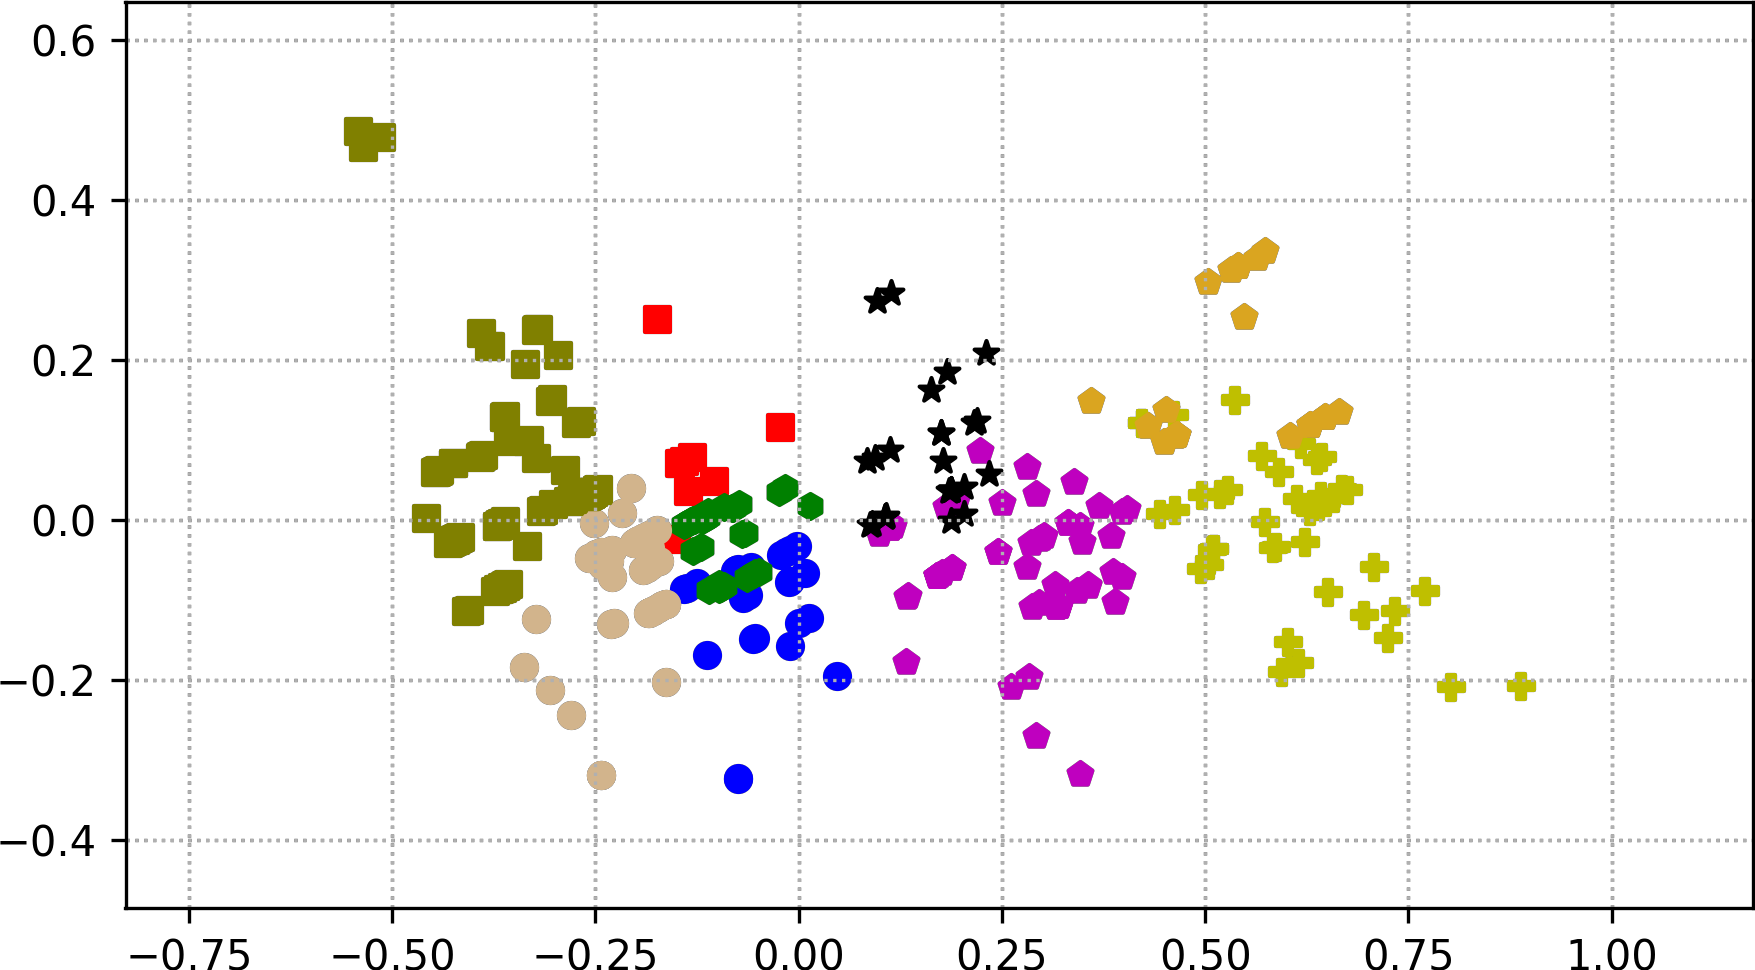
\includegraphics[width=0.45\linewidth]{img/svd/ikmeans-svd}};
	\node[anchor=south west,inner sep=0] (image) at (5.5,3.8) {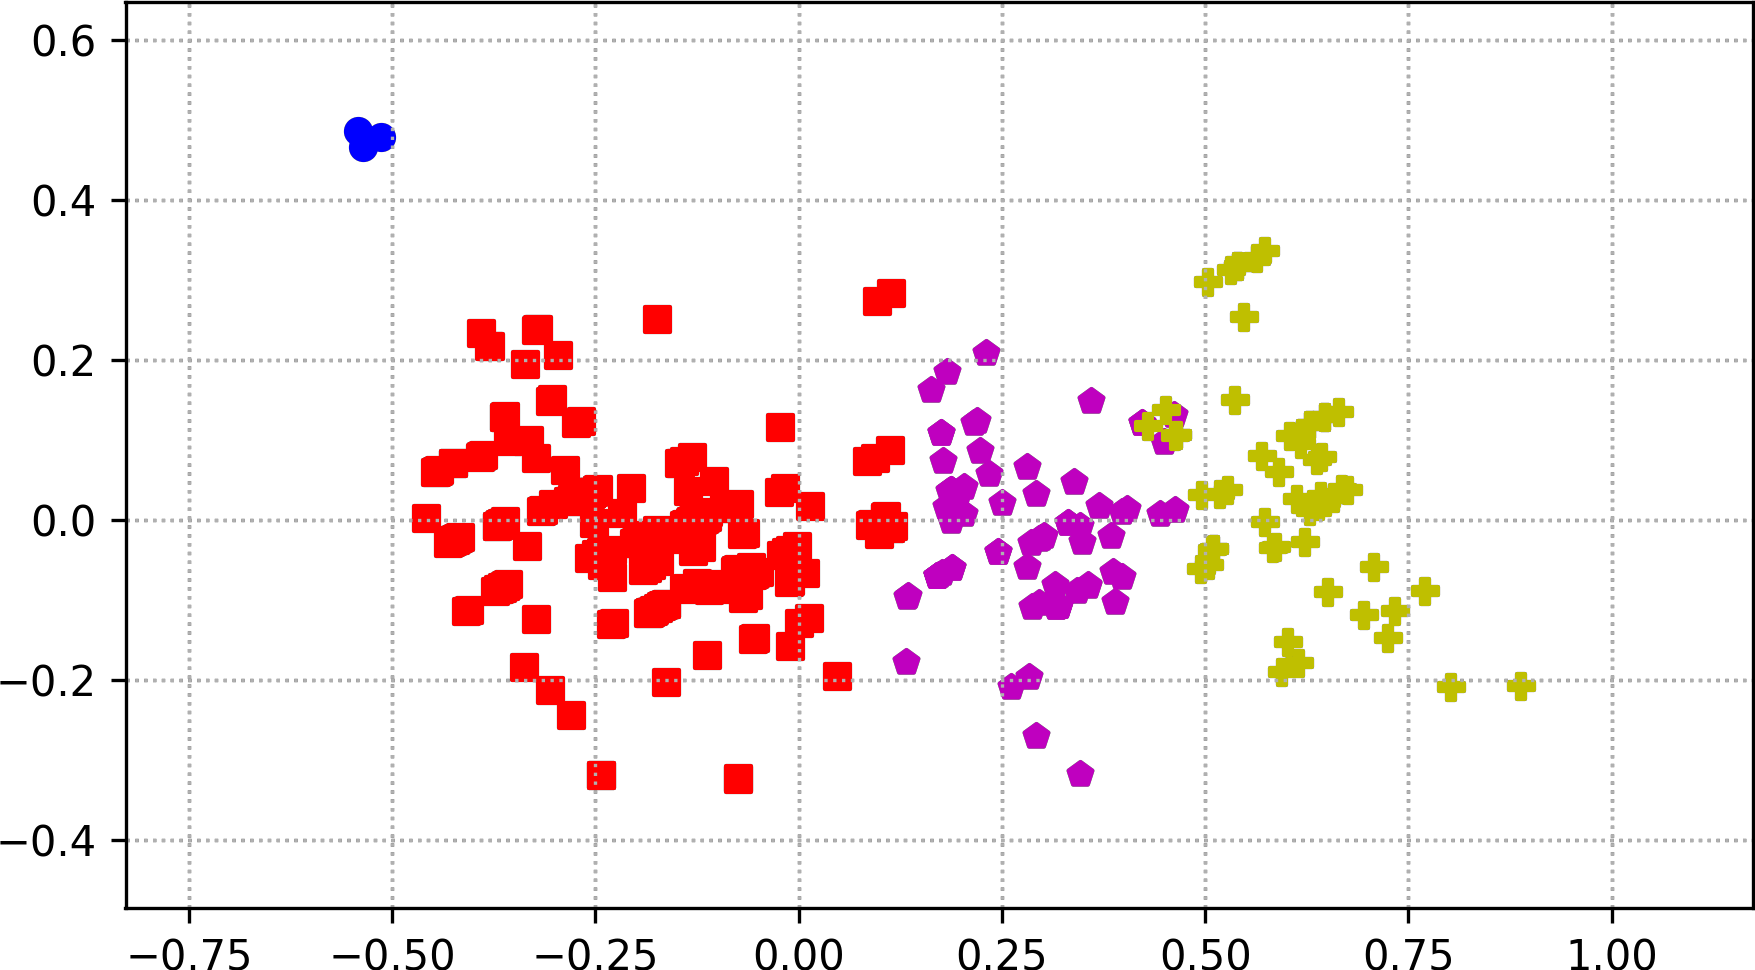
\includegraphics[width=0.45\linewidth]{img/svd/depddp-svd}};
	\node[anchor=south west,inner sep=0] (image) at (-1.5,0) {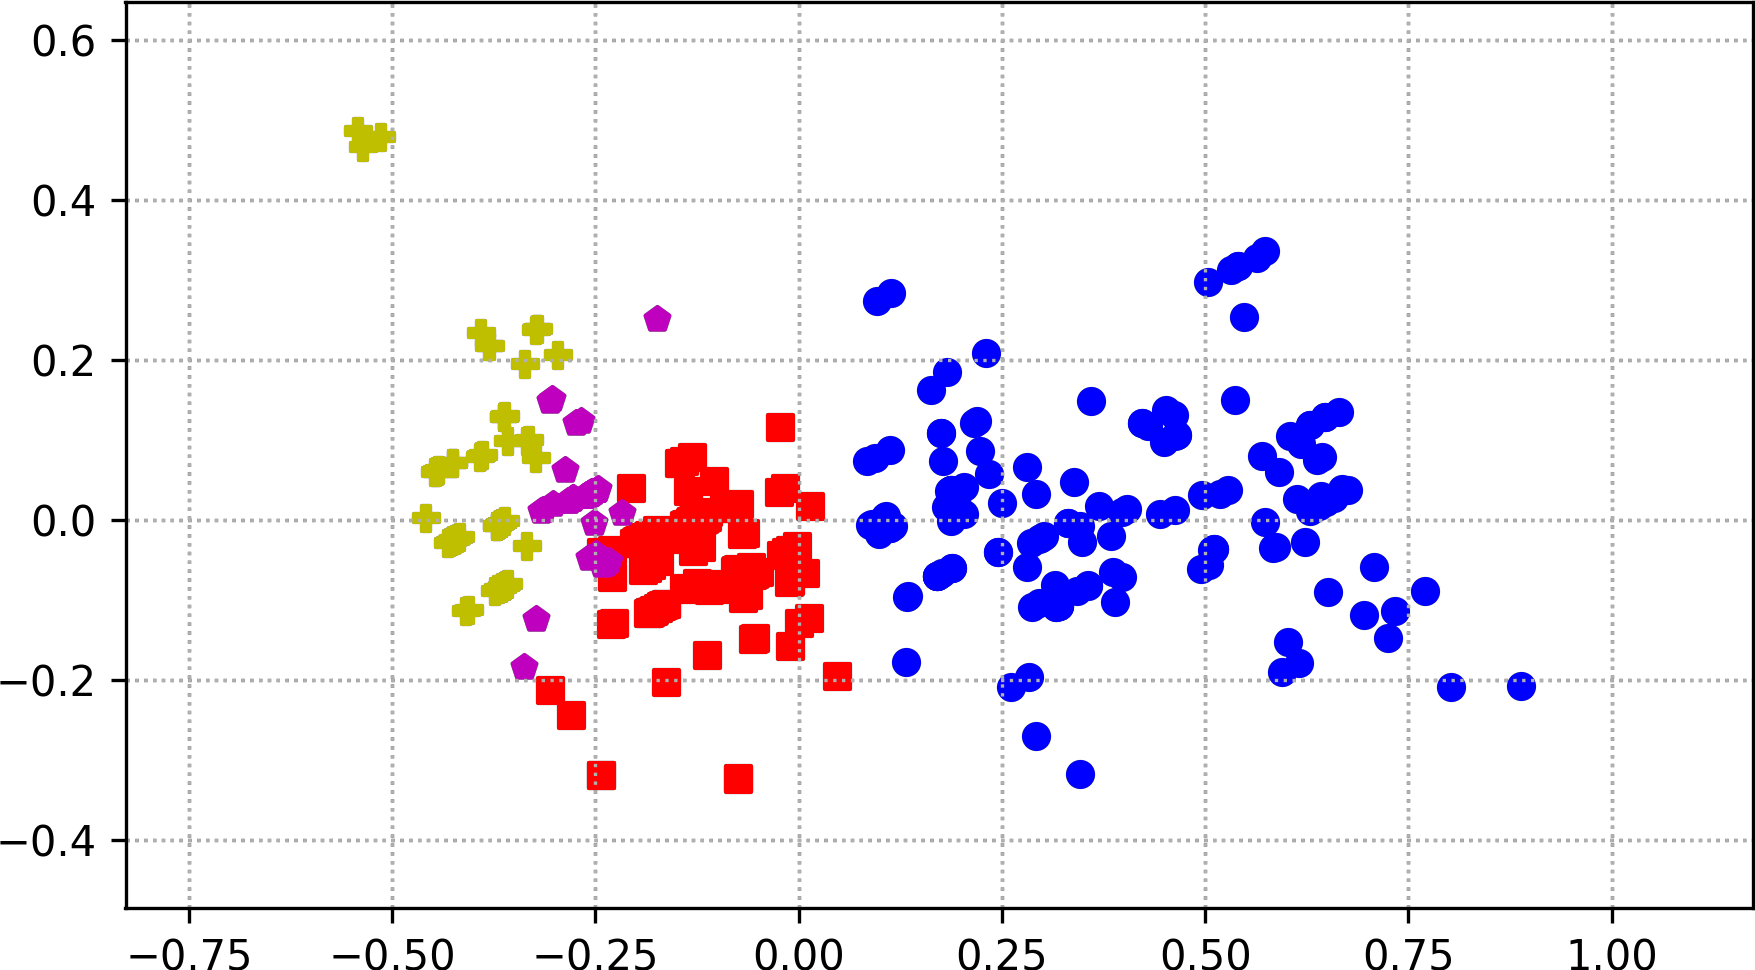
\includegraphics[width=0.45\linewidth]{img/svd/bikmr-svd}};
	\node[anchor=south west,inner sep=0] (image) at (5.5,0) {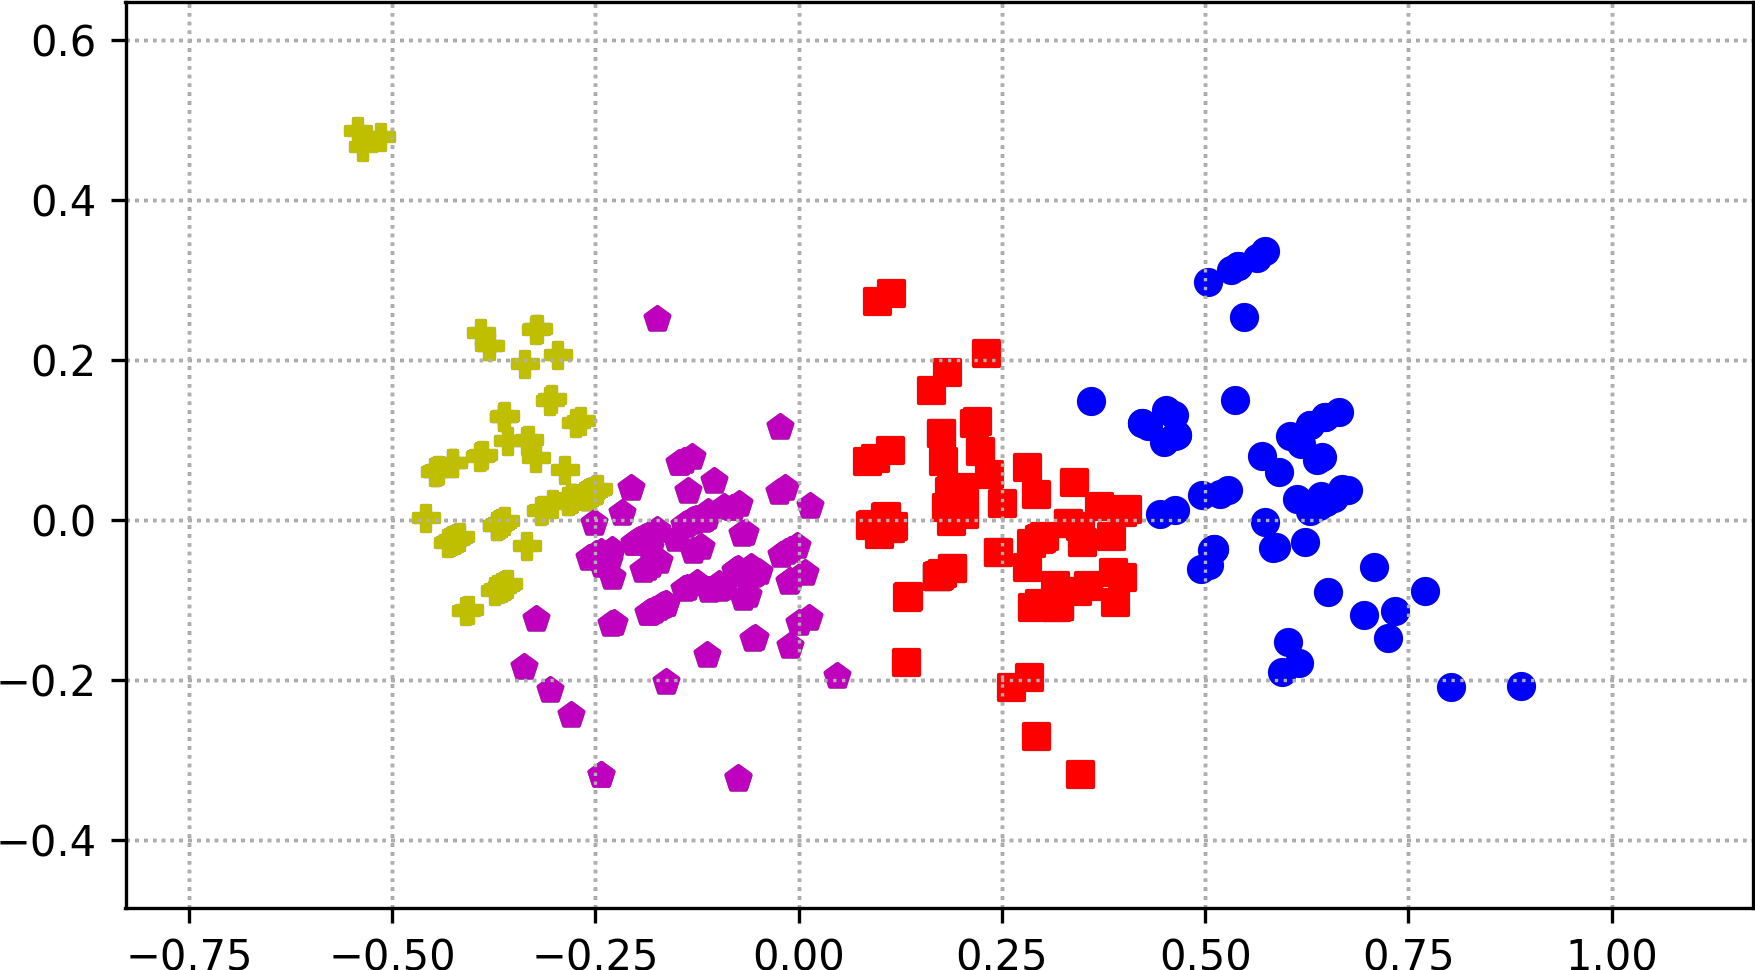
\includegraphics[width=0.45\linewidth]{img/svd/award-svd}};
	\node [draw=none,anchor=west, xshift=0cm, rotate=90,anchor=north,outer sep=-4pt, font=\small, ] at (-1.9,5.5) {\ikmeans (9)};
	\node [draw=none,anchor=west, xshift=0cm, rotate=90,anchor=north,outer sep=-4pt, font=\small, ] at (5.1,5.5) {\dePDDP (4)};
	
	\node [draw=none,anchor=west, xshift=0cm, rotate=90,anchor=north,outer sep=-4pt, font=\small, ] at (-1.9,2) {\BiKMR (4)};
	\node [draw=none,anchor=west, xshift=0cm, rotate=90,anchor=north,outer sep=-4pt, font=\small, ] at (5.1,2) {\AWard (4*)};
	\end{tikzpicture}
	\end{figure}
	\end{frame}

	
	\begin{frame}{Полученное число кластеров}
	\begin{table}[]
	\centering	
	\begin{tabular}{|c|c|}
	\hline
	Число кластеров & Алгоритм \\ 
	\hline
	9 & \ikmeans  \\ 
	\hline
	4  & \dePDDP  \\ 
	\hline
	4   & \BiKMR  \\ 
	\hline
	4*   & \AWard \\
	\hline
	\end{tabular} 
	\end{table}
	\end{frame}

	
	\begin{frame}{Интерпретация}
	\vspace{-0.3cm}
	\begin{center}
	\Large \AWard (наиболее согласованный)\\
	\normalsize
	Отклонения от среднего в каждом кластере в нормализованной шкале (-1...1)
	\end{center}
	\vspace{-0.5cm}
	\begin{figure}[h] % \ContinuedFloat
	\centering
	\includestandalone[width=1\textwidth]{img/tikz/interpretation-award}
	\end{figure}
	\vspace{-0.7cm}		
	\end{frame}


	
	
		
	\plain{	
		\textsc{Выводы}
		\begin{enumerate}
			\item \textbullet~Реализована система, включающая 5 современных алгоритмов 
			\item \textbullet~Для системы INDACT разработана инструкция пользователя
			\item \textbullet~При разработке учтены тенденции в области проектирования ПО
			\item \textbullet~INDACT позволит облегчить применение разработанных алгоритмов 
			\item 
		\end{enumerate}
	}

	\plain{
	\textsc{Спасибо за внимание}!
	}

\end{document}
